\chapter{Mapeamento de Código Limpo em Métricas de Código-fonte}
\label{chap:mapeamento}	

Após a discussão teórica realizada na primeira parte dessa 	monografia, apresentaremos um mapeamento dos conceitos de código limpo em métricas de código-fonte. Nesse mapeamento usamos um conjunto de métricas para automatizar a busca por características do código-fonte. Em seguida, criamos uma interpretação dos valores das métricas, fazendo associações entre eles e as técnicas e conceitos relacionados a limpeza do código. Nosso objetivo é facilitar a detecção de trechos que poderiam sofrer alterações que os tornem mais expressivos, simples e flexíveis.


\section{Métricas de Código-fonte}

Métricas nos permitem criar mecanismos automatizáveis para detecção de características obtidas através da análise do código-fonte. Elas podem ser usadas como pontos de avaliação da qualidade do software \citep{meirelles:sbqs09}. Além disso, No contexto de métodos ágeis, as métricas são importantes parâmetros para \textit{tracking} de projetos (acompanhamento do desenvolvimento do projeto). Por exemplo, contando linhas de código já produzidas, ou no cálculo da cobertura de teste.	
                                                                                       
Nesta monografia usamos uma abordagem baseada na determinação de um conjunto de métricas que seja facilmente interpretado e que visa encontrar trechos de código que precisem de melhorias quanto a sua limpeza.

Partimos do ponto em que sabemos que existem muitas métricas e compreender os significados dos valores de todas é uma tarefa custosa. Essa dificuldade motivou recentemente a criação de ferramentas que automatizam a interpretação dos resultados obtidos. Uma dessas ferramentas é a Kalibro (primeiramente demoninada de Crab), descrita no artigo \citep{meirelles:sbes09}. A mesma permite que o usuário configure intervalos numéricos que possibilitam uma interpretação qualitativa do valor de cada métrica. Assim, podemos usar intervalos como ``Bom'', ``Regular'' e ``Ruim'' ao invés de usar ``0 a 1/3'', ``1/3 a 2/3'' e ``2/3 a 1'', facilitando o entendimento e a classificação dos aspéctos medidos a partir do código-fonte.

No entanto, ao considerar o uso de uma ferramenta como a Kalibro neste trabalho, encontramos algumas dificuldades. Uma é a dependência da combinação de métricas para encontrar as características que procuramos, uma vez que há apenas suporte na Kalibro para interpretação de cada valor separadamente e não para conjuntos deles. Outro problema consiste em como definir os intervalos numéricos. Por exemplo, podemos usar os conceitos apresentados por Robert Martin \citep{Martin2008} para definir essas referências, porém, temos que considerar que diferentes linguagens e domínios de aplicação precisam de padrões de implementação distintos, como comenta Kent Beck \citep{Beck2007}.	

Para evitar esses problemas selecionamos um subconjunto pequeno de métricas que espelha bem as características de código limpo procuradas. A seleção feita não é a única capaz de suprir os mesmos objetivos, pois outras combinações podem ser propostas e obter resultados semelhantes.

Na formação desse subconjunto, a minimalidade não foi uma restrição. Optamos por não eliminar todas as métricas correlacinadas, pois em alguns casos, mesmo que elas indiquem características parecidas, elas nos fornecem alguns outros dados relevantes.

Por fim, dado a dificuldade em fixar valores para a interpretação das métricas, o mapeamento desenvolvido nesta pesquisa não tem como objetivo afirmar se um código é limpo ou não. Nossa proposta é indicar um conjunto de métricas cujos valores expressem diferentes cenários relacionados com melhorias quanto à limpeza do código.
						
	
\section{O Mapeamento}
                    
O mapeamento proposto neste trabalho visa facilitar a procura por problemas quanto a limpeza do código. A ideia é criar cenários que relacionem os conceitos de código limpo com métricas de código-fonte. Cada cenário é descrito através dos seguintes componentes:
	
\begin{itemize}
	\item Conceitos de Limpeza Relacionados: conceitos de limpeza de código que motivaram a criação do cenário.
	\item Características: indicam a presença de falhas em relação as referências apresentadas.
	\item Métricas: mecanismos que permitem analisar o código a procura das características do cenário.
	\item Objetivo Durante a Refatoração: quais devem ser as ideias principais durante a refatoração para eliminar o problema.
	\item Resultados Esperados: quais características devem ser encontradas no código quando terminar a refatoração para eliminação do cenário.
\end{itemize}	


Quando algum cenário é detectado, sugerimos que o usuário analise o trecho indicado, assim verificando se é possível refatorar o código para melhorar sua limpeza. Esse mapeamento não visa afirmar se existem problemas no código, mas sim indicar partes dele que talvez possam ser melhoradas de acordo com os conceitos discutidos nessa trabalho.

Para incentivar a avaliação de códigos ao longo de seu desenvolvimento, é muito importante que sua interpretação seja simples. Esperamos que a preocupação com a limpeza do código não emerja apenas quando ele estiver pronto, pois nessa fase é provável que ele tenha vários problemas e que seja muito complicado alterá-lo. Por esse motivo, montamos alguns cenários e escolhemos um conjunto pequeno de métricas que nos permite detectar as características procuradas.

Até o momento, não conseguimos mapear todos os conceitos de código limpo usando métricas. Por exemplo, não consguimos encontrar problemas relacionados a nomes pouco expressivos usando apenas métricas. Nesse caso, não é suficiente analisarmos somente a estrutura do código, precisaríamos entender o contexto em que cada nome é usado, e para isso, também seria necessária uma análise semântica.

Em suma, existem dois tipos de métricas de código-fonte. Algumas avaliam características de métodos e outras de classes. As métricas de classe são normalmente somas ou médias dos valores das métricas de nível de métodos. Essa divisão de alvo da análise das métricas também existe no contexto dos cenários, que discutiremos adiante.



\subsection{Conjunto de Métricas}

Abaixo apresentamos o conjunto selecionado de métricas.

\subsubsection{NC (\textit{Number of Calls}): Número de Chamadas}

A métrica NC calcula o número de métodos e atributos internos e externos usados por um método. Elementos exeternos são aqueles que pertencem a classes não relacionadas hierarquicamente com a classe da operação analisada. Os internos são os pertencentes a mesma classe.
                                                                 
O valor dessa métrica pode variar entre zero e a soma do número de atributos e métodos presentes no sistema. Obtemos zero quando o método em análise não acessa nenhum atributo e não faz chamadas a métodos.
	

\subsubsection{NEC (\textit{Number of External Calls}): Número de Chamadas Externas}

A métrica NEC calcula o número de métodos e atributos externos acessados por um método. Definimos como externos os elementos pertencentes a classes não relacionadas hierarquicamente com a classe do método em análise.
 	                                               
NEC é uma adaptação da métrica ATFD (\textit{Access To Foreing Data} \citep{Marinescu02}) que calcula o número de atributos de classas não relacionadas que são acessados diretamente ou através de chamadas a métodos de acesso. 

Seu valor pode variar de zero até o número total de métodos e atributos do sistema. Nesse caso, zero indica que não há comunicação entre o método e qualquer outra classe sem relação com a sua.
	        
Calculamos a média de NEC quando precisamos avaliar o número médio de chamadas de métodos e acessos a atributos externos por método de uma classe. 
                                                                                                           
                          
\subsubsection{ECR (\textit{External Calls Rate}): Taxa de Chamadas Externas}
                                         
A métrica ECR calcula a taxa de chamadas externas realizadas por um método. Para isso, são necessários o número de chamadas externas (NEC) e o total de chamadas (NC) realizadas pelo método. O valor da taxa será o resultado da divisão de NEC por NC.

Essa métrica é uma adaptação da LAA (\textit{Locality of Attribute Accesses} \citep{Lanza06}) que calcula o número de atributos pertencentes a mesma classe que o método em análise, dividido pelo número total de variáveis acessadas (incluindo atributos usados através de métodos de acesso). 

Seu valor varia entre zero e um. Obtemos zero quando o método não possui chamadas externas e um quando todas as chamadas realizadas são externas.


\subsubsection{NCC (\textit{Number of Classes Called}): Número de Classes Chamadas}              

A métrica NCC calcula o número de classes das quais métodos são chamados ou atributos são acessados por um método. Nesse calculo não contamos classes que tenham relação hierarquica  com a classe do método em análise.

Essa métrica é uma adaptação da FDP (\textit{Foreign Data Providers} \citep{Lanza06}) que calcula o número de classes das quais atributos são acessados. Seu valor varia entre zero e o número total de classes do sistema. Obtemos zero quando o método não utiliza elementos de outras classes.
                                                                 

\subsubsection{NRA (\textit{Number of Reachable Attributes}): Número de Atributos Alcançáveis}

A métrica NRA calcula o número de atributos alcançáveis a partir de um método. Um atributo pode ser alcançado direta ou indiretamente. O acesso é direto quando o atributo é usado no próprio corpo do método, e é indireto quando existe uma chamada para algum método que usa o atributo direta ou indiretamente.
 	          
Para descobrirmos quantos atributos são alcançáveis por um método, podemos criar um grafo com atributos e métodos como vértices e os acessos e chamadas a eles como arestas. Com esse grafo criado, podemos encontrar os vértices atingíveis a partir do vértice que representa o método em análise. Então, contamos quantos deles são atributos. E assim, obtemos o número de atributos alcançáveis pelo método.

O valor dessa métrica varia entre zero e o total de atributos da classe do método. Obtemos zero quando o método não alcança nenhum atributo de sua classe e o valor máximo quando ele usa direta ou indiretamente todos os atributos de sua classe.


\subsubsection{MaxNesting (\textit{Maximum Nesting Level}): Nível Máximo de Estruturas Encadeadas}

A métrica MaxNesting \citep{Lanza06} calcula o nível máximo de estruturas encadeados presentes no corpo de um método.

Seu valor varia entre zero e a quantidade total de quebras de fluxo do método. Obtemos zero quando o método não possui controladores de fluxo. Atingimos o valor máximo quando todas as quebras condicionais presentes no método encontran-se em níveis diferentes da mesma estrutura.

Os comandos \textit{if}, \textit{while} e \textit{for} são alguns exemplos de controladores de fluxo bastante usados em diversas linguagens.
                         

\subsubsection{CYCLO \textit{Cyclomatic Complexity}: Complexidade Ciclimática}

A métrica CYCLO \citep{McCabe76} calcula o número de caminhos linearmente independentes no método analisado, conhecido como complexidade ciclomática.

Seu valor mínimo é um e não existe um limite máximo para o seu resultado. Obtemos um quando não há quebra do fluxo principal. Cada estrutura de controle de fluxo presente no corpo do método adiciona um no valor total da CYCLO.
	                          
Quando os valores de MaxNesting e CYCLO são próximos, sabemos que muitos dos controladores de fluxo presentes no método estão encadeados em uma mesma estrutura. Quando são muito distantes, podemos concluir que os controladores estão espalhados em estruturas diferentes e que elas não são muito profundas.
                                   

\subsubsection{NP: Número de Parâmetros}

A métrica NP calcula o número de parâmetros de um método. Seu valor mínimo é zero e não existe um limite máximo para o seu resultado. Obtemos zero quando o método avaliado não possui parâmetros.
                                                             
Calculamos a média de NP quando precisamos avaliar a média do número de parâmetros por método de uma determinada classe.	   
                                   

\subsubsection{NRP: Número de Repasses de Parâmetros}

A métrica NRP calcula o número de parâmetros recebidos pelo método em análise e repassados como argumento em chamadas a outras operações pertencentes a sua classe.                                                    
	
Seu valor varia entre zero e o número de parâmetros do método (indicado pela métrica NP). Obtemos zero quando nenhum parâmetro é repassado. O valor máximo é atingido quando todos os parâmetros são usados como argumentos em alguma chamda de operção realizada no corpo do método. 
                              
Calculamos a média de NRP quando precisamos avaliar a média do número de repasses de parâmetros por método de uma classe.
                        
                                                             
\subsubsection{LOC (\textit{Lines of Code}): Número de Linhas}

A métrica LOC \citep{LK94} calcula o número de linhas efetivas de um método. Linhas compostas apenas por comentários ou vazias não são consideradas efetivas.
 

\subsubsection{NOA (\textit{Number of Attributes}): Número de Atributos}

A métrica NOA calcula o número de atributos de uma classe. Seu valor mínimo é zero e não existe um limite máximo para o seu resultado. Obtemos zero quando a classe analisada não possui atributos.
                         

\subsubsection{NOM (\textit{Number of Methods}): Número de Métodos}

A métrica NOM calcula o número de métodos de uma classe. Seu valor mínimo é zero e não existe um limite máximo para o seu resultado. Obtemos zero quando a classe não possui métodos.                                                                   
                           
                                                        
\subsubsection{SLOC: Soma do Número de linhas}
                                          
A métrica SLOC calcula a soma do número de linhas efetivas de todos os métodos de uma classe. Ou seja, seu resultado é a soma dos valores do LOC de cada método da classe.


\subsubsection{AMLOC: Média do Número de Linhas Por Método}
                                   
AMLOC calcula a média do número de linhas efetivas por método da classe analisada.
	

\subsubsection{LCOM4 (\textit{Lack of Cohesion}): Falta de Coesão Entre Métodos}

A métrica LCOM4 \citep{HM96} calcula a falta de coesão da classe analisada. Para isso, é montado um grafo cujos vértices são os atributos e métodos da classe. Cada aresta desse grafo representa o acesso de um atributo ou a chamada de método através de um outro método. Quando o grafo estiver pronto, são contabilizados os componentes conexas existem nele. Esse número indica a quantidade de subconjuntos em que a classe está dividida.

Seu valor mínimo é um e não existe um limite máximo para o seu resultado. Obtemos um quando a classe não possui subdivisões, ou seja, quando a classe é bastante coesa. Normalmente, desejamos classes que não possuem conjuntos isolados de métodos e atributos, pois o número de subdivisões costuma indicar a quantidade de classes que deveriam existir para que cada uma fosse responsável por apenas um contexto.
                                                    
	  

\subsection{Os Cenários}

\subsubsection{Método Grande}

Os conceitos tratados no Cápitulo de Código Limpo que constituem este cenário, denominado de Métodos Grandes, são: composição de métodos, a necessidade de evitar estruturas encadeadas e, a possibilidade de usar cláusula guarda.
	
Nesse contexto, métodos grandes tem como principal característica (i)um elevado número de linhas, ou seja, um alto valor de LOC. É comum também possuir (ii) um elevado número de quebras condicionais de fluxo, indicado por um valor alto da CYCLO e (iii) profundas estruturas com condicionais encadeados, indicadas por um valor alto do MaxNesting.
                                               
Durante uma refatoração deste cenário, nosso objetivo é diminuir o número de linhas (LOC), diminuir a complexidade ciclomática (CYCLO) e eliminar as estruturas encadeadas (MaxNesting) no método em análise. Conseguimos atingir esses obejetivos decompondo o método grande em métodos menores. Normalmente começamos essa decomposição passando os blocos de código dos desvios de fluxo para outros lugares, pois esses são conjuntos de operações evidentemente isoladas do resto do método.
                                                
Após a refatoração de todas as ocorrências deste cenário na classe em análise, esperamos que a sua média de linhas por método (média de LOC) e as profundidades máximas de estruturas encadeadas de cada método (MaxNesting) abaixem. Provavelmente a complexidade ciclomática da classe (CYCLO) não sofrerá alterações. Isso acontece porque normalmente espalhamos essas quebras de fluxo em outros métodos da mesma classe, mas não as eliminamos da sua lógica. Teremos uma redução da complexidade ciclomática quando parte do código for eliminado ou trasferido para métodos de outras classes. Além disso, pode acontecer um aumento no número de métodos da classe, um aumento do número de métodos de outras classes ou até a criação de novas classes.

Possuir muitas funcionalidades e parâmetros são mais duas características deste cenário. Porém, não precisamos nos preocupar com elas diretamente. Suas quantidades serão reduzidas como consequência da refatoração baseada nos outros aspéctos citados.

Para exemplificar este cenário, vamos analisar o método \textit{custosAPartirDoVertice} (trecho de código \ref{metodo_grande}). Nessa avaliação, devemos calcular os valores das métricas que indicam a presença das características do problema descrito. 
                                                                                                                         
\lstinputlisting[label=metodo_grande, caption={O método custosAPartirDoVertice é um exemplo de método grande}]{codigos/exemplos_para_os_cenarios/metodo_grande}                                                            

Quando contamos o número de linhas efetivas desse método, obtemos \textit{LOC = 17}. Ao contabilizar a quantidade de controladores de fluxo, chegamos a \textit{CYCLO = 6}. Por fim, temos que a profundidade máxima entre as estruturas de controladores encadeados, medida por MaxNesting, é igual a 4. Baseado no príncipio de procurarmos métodos pequenos, esses valores podem ser indícios de que esse método possui problemas relacionados a limpeza de código por ter características de um método grande.
                                                      
O trecho de código \ref{refatoracao_para_metodo_grande} é uma possível refatoração para o método \textit{custosAPartirDoVertice}. Nesse caso, reduzimos a quantidade de responsabilidades do método, passando-as para outros métodos menores: \textit{inicializaCustosEFila} e \textit{atualizaCustosAteAcabarVertices}. Esses métodos também são pequenos pois quebram suas tarefas e as passam para outras operações que seguirão esse mesmo princípio. Quando calculamos as métricas deste cenário no método refatorado, obtemos \textit{LOC = 3}, \textit{CYCLO = 1} e \textit{MaxNesting = 0}. Comparando com os resultados antigos, podemos observar uma grande redução nos valores após a refatoração. Dados os novos resultados, podemos dizer que o método \textit{custosAPartirDoVertice} não está mais no cenário de método grande.

\lstinputlisting[label=refatoracao_para_metodo_grande, caption={Uma possível refatoração para o método custosAPartirDoVertice deixar de ser um método grande}]{codigos/exemplos_para_os_cenarios/refatoracao_para_metodo_grande}                                                            

	
\subsubsection{Método com Muitos Fluxos Condicionais}
                  
Os conceitos de código limpo que constituem este cenário são a composição de métodos e o uso de exceções. Esse cenário ocorre quando temos métodos que são complexos, mas não necessariamente grandes. Suas principais característica são: (i) muitas quebras condicionais de fluxo (valor alto da CYCLO) e (ii) longas estruturas com condicionais encadeados (valor alto de MaxNesting).
                                                                                 
Durante uma refatoração deste cenário, buscamos minimizar a complexidade ciclomática (CYCLO) e a profundidade máxima de estruturas encadeadas (MaxNesting) do método, pois queremos deixar o código mais simples e direto. Podemos nos basear na decomposição de métodos para atingirmos nossos objetivos.
	
Depois das modificações, esperamos que o a profundidade máxima de estruturas encadeadas tenha diminuído (redução do MaxNesting). Quando a refatoração for baseada no uso de exceções, como \textit{try catch} é provável que a complexidade ciclomática do método não se altere, pois essas estruturas também são contadas como desvios de fluxo no calculo da CYCLO. Pode acontecer também um aumento no número de métodos da classe, porque, em alguns casos, o conteúdo do bloco de cada desvio condicional é deslocado para novos métodos. 
           
Para exemplificar este cenário, usaremos o método \textit{deletaPaginasETodasAsReferencias} (trecho de código \ref{metodo_com_muitos_fluxos_condicionais}). Quando analisamos esse bloco de código usando as métricas indicadas neste cenário, encontramos os valores \textit{CYCLO} = 4 e \textit{MaxNesting} = 3. Se condideramos esses valores com indícios de que temos muitos controladores de fluxo e uma longa estrutura desses controladores encadeados, podemos dizer que esse método tem muitos fluxos condicionais. 
                                                                                          
\lstinputlisting[label=metodo_com_muitos_fluxos_condicionais, caption={O método deletaPaginasETodasAsReferencias é um exemplo de método com muitos fluxos condicionais}]{codigos/exemplos_para_os_cenarios/metodo_com_muitos_fluxos_condicionais}               
                                                                                          
Analisando o código a procura de possíveis refatorações, observamos que esse método realiza três operações e a verificação de falha para cada uma delas. Esse tratamento de erros poderia ser feito usando \textit{try catch}. Essa mudança diminuiria o valor de \textit{MaxNesting} e de \textit{CYCLO}, reduzindo o problema encontrado. O resultado dessa refatoração é o método exposto no trecho de código \ref{uso_de_try_catch_no_problema_com_fluxos_condicionais}.
                                                         
\lstinputlisting[label=uso_de_try_catch_no_problema_com_fluxos_condicionais, caption={Uma refatoração usando \textit{try catch} para o método deletaPaginasETodasAsReferencias}]{codigos/exemplos_para_os_cenarios/uso_de_try_catch_no_problema_com_fluxos_condicionais}
              
Com essa refatoração deixamos o método mais simples e fora deste cenário.


\subsubsection{Método com Muitos Parâmetros}
                                                                         
Este cenário tem como base o conceito de agrupamento de parâmetros em objetos. A principal característica de um método que está nesse contexto é ter um elevado número de parâmetros (valor alto de NP).
                                                         
Durante uma refatoração desse cenário, o objetivo é minimizar o número de parâmetros recebidos (diminuir o NP). Os resultados esperados após a refatoração são a redução do número de parâmetros (NP) e o aumento do número de classe. Esse aumento ocorre quando criamos classes para agrupar os parâmetros que pertencem a um mesmo contexto em um único objeto.
	                                               
Para exemplificar este cenário, usaremos o método \textit{calculaQuantidadeDeDias} (trecho de código \ref{metodo_com_muitos_parametros}). Quando calculamos sua quantidade de parâmetros, obtemos \textit{NP = 6}. Esse valor pode ser considerado alto para a métrica NP, assim é factível dizer que esse método está no contexto de método com muitos parâmetros.                    	

\lstinputlisting[label=metodo_com_muitos_parametros, caption={O método calculaQuantidadeDeDias é um exemplo de método com muitos parametros}]{codigos/exemplos_para_os_cenarios/metodo_com_muitos_parametros}                   
                                                                                                        
Ao analisarmos os parâmetros presentes nesse exemplo, podemos notar que eles representam duas datas formadas por \textit{dia, mês e ano}, que indicam o início e o fim de um período. Então, uma refatoração possível para esse código seria criar uma classe \textit{Data} da qual cada objeto representasse uma dessas datas. Assim, reduziríamos o valor de \textit{NP} de seis para dois, eliminando o problema de alto número de parâmetros desse método (trecho de código \ref{refatoracao_para_metodo_com_muitos_parametros}). 
                                                                               
\lstinputlisting[label=refatoracao_para_metodo_com_muitos_parametros, caption={O método calculaQuantidadeDeDias depois da refatoração para redução do número de parâmetros}]{codigos/exemplos_para_os_cenarios/refatoracao_para_metodo_com_muitos_parametros}          
              

\subsubsection{Muita Passagem de Parâmetros Pela Classe}
	
Este é o primeiro cenário que descrevemos relacionado com a avaliação da classe como um todo e não de métodos separados. Os conceitos de código limpo que constituem este cenário são o agrupamento de parâmetros em objetos e a transformação de parâmetros em variáveis de instância.
	
Podemos separar esse cenário em dois casos diferentes. O primeiro trata do repasse de muitos parâmetros. Sua característica é ter uma elevada média de parâmetros repassados (alta média de NRP). Parâmetros repassados são aqueles recebidos por um método que os repassam em chamadas a operações. O segundo caso se preocupa com a elevada média do número de parâmetros por método da classe analisada (alta média de NP).       
		     
Então, é comum que os métodos de classes com muita passagem de parâmetro tenham muitos ou repassem muitos parâmetros, ou recebam variáveis que são usadas apenas em chamadas a outros métodos.	O método \textit{acumulaRelatorioDasMetricasGlobais} (trecho de código \ref{metodo_com_muito_repasse_de_parametros}) exemplifica a existência de parâmetros que são apenas repassados em chamadas a outras operações. Os três parâmetros desse exemplo (\textit{totaisDasMetricasDeModulo}, \textit{contagensDeModulo} e \textit{listaDeValores}) possuem essa característica. 
	                                                               
\lstinputlisting[label=metodo_com_muito_repasse_de_parametros, caption={O método custosAPartirDoVertice é um exemplo de método com muito repasse de parâmetros}]{codigos/exemplos_para_os_cenarios/metodo_com_muito_repasse_de_parametros}                                     
	
Os objetivos durante uma refatoração deste cenário são diminuir o número de repasses de parâmetros pela classe (diminuir o NRP) e reduzir o número de parâmetros dos métodos (reduzir o NP). Fazemos isso tranformando os parâmetros muito repassados ou usados em vários métodos em atributos e criando objetos para guardar conjuntos de parâmetros relacionados.
	
Os resultados esperados após a refatoração do código são a redução da média do número de parâmetros por método (redução da média de NP), redução do número de repassagem de parâmetro (redução do NP) e o aumento do número de variáveis de instância. Além disso, pode ocorrer um aumento no número de classes caso aconteça a junção de variáveis em um único objeto.	           


\subsubsection{Método ``Invejoso''}
\label{cenario_metodo_invejoso}

Método ``invejoso'' é aquele que usa um elevado número de métodos e atributos de poucas classes não relacionadas hierarquicamente com a sua própria. Mapeando essas características em métricas de código-fonte, temos neste cenário alta ECR, que indica a taxa de chamadas a métodos e atributos externos, e baixa NCC, que representa o número de classes não relacionadas chamadas pelo método.
	
A preocupação durante uma refatoração neste contexto, deve ser a minimização do número de chamadas externas, calculado através do NEC. O conceito de código limpo que constitui este cenário é a delegação de tarefa.
	
Após a refatoração, esperamos uma redução do número de chamadas externas (diminuição do NEC), da taxa de chamadas externas (diminuição do ECR) e da média do número de chamadas externas da classe (diminuição da média de NEC).
                      
Para exemplificar este cenário, usaremos o método \textit{salarioDoMes} da classe \textit{CalculaReceita} (trecho de código \ref{metodo_invejoso}). Quando calculamos a taxa de chamadas externas realizadas por esse método, obtemos \textit{ECR = NEC/NC = 4/4 = 1}. O resultado é o valor máximo para essa métrica, o que indica que o método possui apenas chamadas externas e que, portanto, tem alto acoplamento. Devemos, então, calcular a quantidade de classes diferentes que são chamadas por esse método. O resultado é \textit{NCC = 1}. Esse valor indica que todos os elementos externos usados são da mesma classe. Como a taxa de chamadas externas é alta e todos os elementos externos usados são da mesma classe, podemos dizer que o método \textit{salarioDoMes} está no cenário de método ``invejoso''.

\lstinputlisting[label=metodo_invejoso, caption={Método salarioDoMes com problemas de ``inveja''}]{codigos/exemplos_para_os_cenarios/metodo_invejoso}                                      

Para resolver esse problema, podemos passar para a classe empregado o método \textit{salarioDoMes} (trecho de código \ref{refatoracao_para_metodo_invejoso}). Quando isso acontecer os valores das suas métricas serão \textit{ECR = NEC/NC = 0/4 = 0} e \textit{NCC = 0}, o que resolve o seu problema de ``inveja'' dada a redução do acoplamento entre as classes \textit{CalculaReceita} e \textit{Empregado}. 

\lstinputlisting[label=refatoracao_para_metodo_invejoso, caption={Redução do acoplamento entre as classes CalculaReceita e Empregado}]{codigos/exemplos_para_os_cenarios/refatoracao_para_metodo_invejoso}


\subsubsection{Método Dispersamente Acoplado}
\label{cenario_metodo_dispersamente_acoplado}	

Um método dispersamente acoplado utiliza um elevado número de atributos e métodos de várias classes não relacionadas hierarquicamente com a sua. Assim como no contexto de método ``invejoso'', nesse cenário temos um valor alto de ECR, indicando que o uso de métodos e atributos externos é maior do que de internos. Porém, a diferença entre eles é o número de classes não relacionadas chamadas pelo método, sendo o valor do NCC alto nesse cenário e baixo para métodos ``invejosos''.
	
Durante uma refatoração, devemos focar na redução do número de chamadas externas que é calculado através da métrica NEC. Os conceitos de código limpo que constituem este cenário são o de objeto centralizador e o de objeto método.
	
Os resultados esperados após a refatoração são a redução do número de chamadas externas e de sua média na classe do método analisado (NEC e média de NEC) e a diminuição do número de classes não relacionadas chamadas (NCC). Também pode ocorrer um aumento no número de classes. Isso acontecerá quando uma classe for criada para centralizar o diálogo entre as classes não relacionadas, sendo sacrificado para que as outras mantenham suas características e sejam reutilizáveis em outros projetos. 
	  
Para exemplificar este cenário, usaremos o método \textit{adicionaDadosDaRodada} (trecho de código \ref{metodo_dispersamente_acoplado}). Quando o avaliamos usando as métricas \textit{ECR} e \textit{NCC} obtemos valores elevados, pois nesse código são usados seis métodos externos de quatro classes diferentes. Com esses resultados dizemos que esse método é dispersamente acoplado.
  
\lstinputlisting[label=metodo_dispersamente_acoplado, caption={Método ``adicionaDadosDaRodada'' dispersamente acoplado}]{codigos/exemplos_para_os_cenarios/metodo_invejoso}                                      
                      

\subsubsection{Classe Pouco Coesa}
    
Os conceitos de código limpo que constituem este cenário são a maximização da coesão e o princípio da responsabilidade única. Assim como o cenário que indica muita passagem de parâmetros pela classe, esse contexto analisa a classe como um todo.
	
A principal característica de uma classe pouco coesa é possuir subdivisões em grupos de métodos e atributos que não se relacionam (valor de LCOM4 > 1), ou possuir métodos que alcançam em média poucos atributos da propria classe (média de NRA muito menor do que o valor de NOA). Nesse contexto, dizemos que um método alcança um atributo se ele usa o atributo no seu próprio corpo ou de forma indireta, ou seja, através da chamada de algum método que usa o atributo direta ou indiretamente.


\begin{figure}[htb]
	\centering
	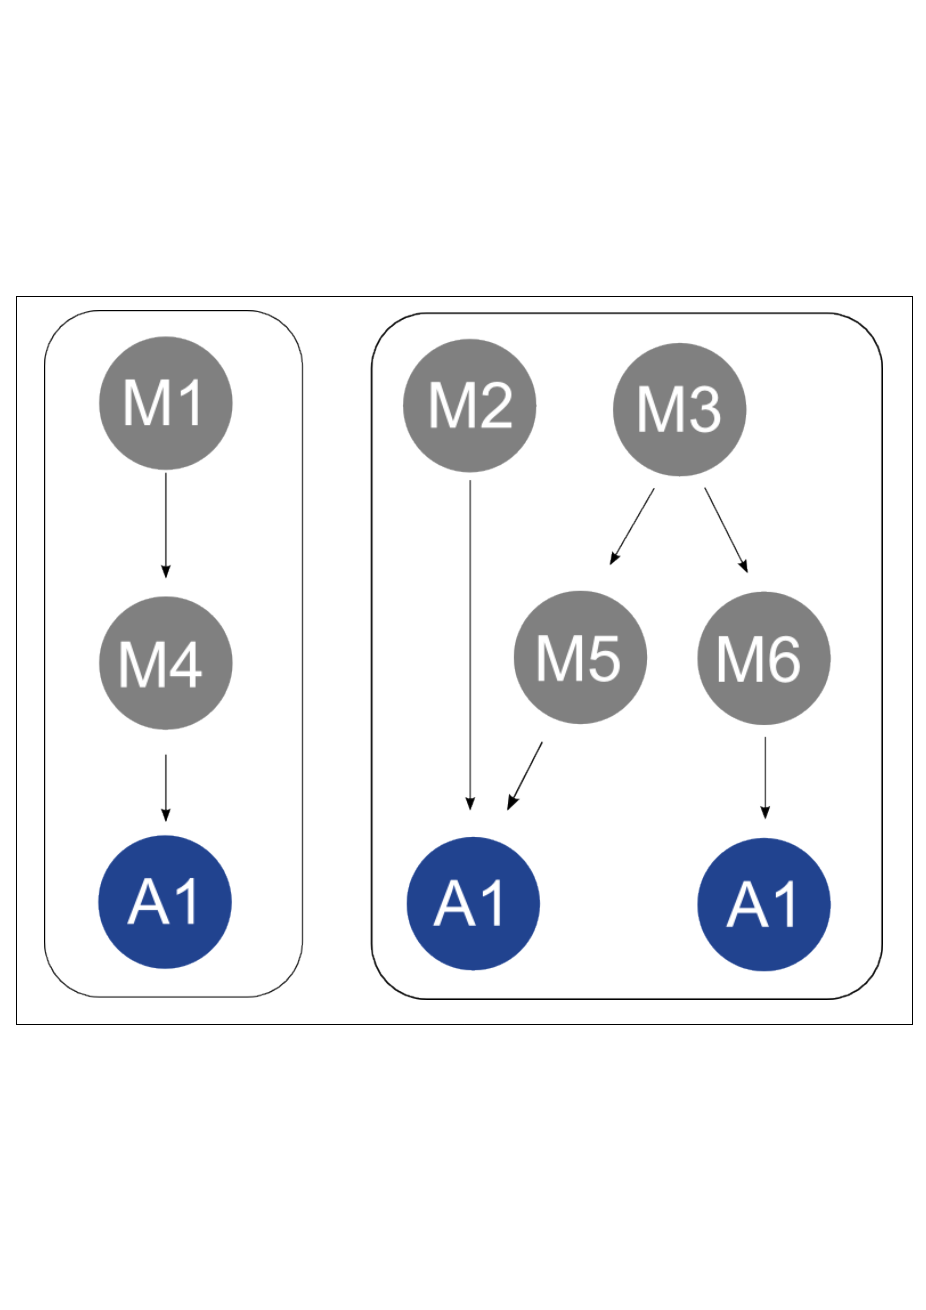
\includegraphics[trim = 0mm 50mm 0mm 60mm, clip, width=0.4\textwidth]{codigos/exemplos_para_os_cenarios/classe_pouco_coesa.png}
	\caption{Representação abstrata de uma classe pouco coesa}
	\label{classe_pouco_coesa}
\end{figure}
   
    
Na figura acima temos a representação abstrata de uma classe. Os círculos cinzas são os métodos e os azuis atributos da classe. As setas representam chamadas e acessos entre esses elementos. Quando contamos os grupos de elementos conexos, obtemos \textit{LCOM4 = 2}, e no cálculo do número médio de atributos atingidos por cada método, obtemos \textit{média de NRA = 1.16}. Como o valor de \textit{LCOM4} é maior do que um e o de \textit{NRA} é razoavelmente menor do que o número total de atributos (\textit{NOA = 3}), podemos classificar essa classe como pouco coesa.                  
    
Os objetivos durante uma refatoração deste cenário são aumentar a coesão (diminuir a LCOM4) e diminuir a diferença entre média do número de atributos alcançáveis (NRA) e o número de atributos da classe analisada (NOA). Portando, uma boa refatoração neste contexto seria separar as subdivisões já existentes na classe analisada em classes mais coesas.
	
Como resultado da refatoração deste cenário, esperamos encontrar um aumento do número de classes. Além disso, desejamos que as classes existentes não tenham subdivisões (LCOM4 = 1) e que a média do número de atributos alcançáveis por cada método seja próxima da quantidade de atributos da classe (média de NRA próxima de NOA).
                  
                
                           
\section{Resumo dos Cenários}

A tabela abaixo resume os cenários apresentados ao longo deste capítulo.

\newenvironment{my_table}
{\begin{list}{\labelitemi}
{  \setlength{\itemsep}{0pt}
  \setlength{\parskip}{0pt}
  \setlength{\parsep}{0pt}
  \setlength{\topsep}{0pt}
  \setlength{\partopsep}{0pt}
  \setlength{\leftmargin}{1em}
  \setlength{\rightmargin}{0.5em}
  \setlength{\topmargin}{0.5em}
}
}
{\end{list}}    

\begin{landscape}

\begin{table}[hbt]

\scalefont{.8}        
\begin{tabular}{|p{3cm}|p{4.5cm}|p{5.0cm}|p{5.5cm}|p{5.0cm}|}
\hline 
\textbf{Cenário} & \textbf{Conceitos de Limpeza} & \textbf{Características} & \textbf{Objetivos Durante a Refatoração} & \textbf{Resultados Esperados} \tabularnewline
\hline
                     

\hline 
Método Grande                           
& \begin{my_itemize}
    \item Composição de Métodos
	\item Evitar Estruturas Encadeadas
	\item Uso de Cláusula Guarda
  \end{my_itemize}
& \begin{my_itemize}
	\item Grande número de linhas efetivas (alto LOC)
	\item Muitas estruturas controladoras de fluxo (alto CYCLO)
	\item Muitas estruturas controladoras de fluxo encadeadas (alto MaxNesting)   
   \end{my_itemize}
& \begin{my_itemize}
	\item Reduzir LOC do método
	\item Reduzir complexidade ciclomática (CYCLO)
	\item Reduzir MaxNesting
  \end{my_itemize}
& \begin{my_itemize}
	\item Redução da média de LOC por método da classe
	\item Não há alteração da complexidade ciclomática (CYCLO) da classe
	\item Redução do MaxNesting dos métodos da classe
  \end{my_itemize}
\tabularnewline
      
\hline 
Método com Muitos Fluxos Condicionais                           
& \begin{my_itemize}
    \item Composição de Métodos
	\item Uso de Exceções
  \end{my_itemize}
& \begin{my_itemize}
	\item Muitas estruturas controladoras de fluxo (alto CYCLO)
	\item Muitas estruturas controladoras de fluxo encadeadas (alto MaxNesting)   
   \end{my_itemize}
& \begin{my_itemize}
	\item Reduzir complexidade ciclomática do método (CYCLO)
	\item Reduzir MaxNesting
  \end{my_itemize}
& \begin{my_itemize}
	\item Redução do MaxNesting dos métodos da classe
	\item OBS:
		\item[-] a complexidade ciclomática pode não reduzir, pois, em alguns casos, o uso de try catch mantêm a quantidade de quebra de fluxo.         
		\item[-] pode acontecer um aumento no número de métodos da classe quando criamos um método separado para cada quebra de fluxo do código.
  \end{my_itemize}
\tabularnewline                          
       
\hline 
Método com Muitos Parâmetros                         
& \begin{my_itemize}
    \item Objeto como Parâmetro
  \end{my_itemize}
& \begin{my_itemize}                            
    \item Elevado número de parâmetros (alto NP)
   \end{my_itemize}
& \begin{my_itemize}
	\item Minimizar o número de parâmetros (NP)
  \end{my_itemize}
& \begin{my_itemize}                           
	\item Redução do número de parâmetros (NP)
	\item Aumento do número de classes
  \end{my_itemize}
\tabularnewline                              

\hline 
Muita Passagem de Parâmetros na Classe                         
& \begin{my_itemize}
    \item Objeto como Parâmetro
	\item Parâmetros como Variáveis de Instância
  \end{my_itemize}
& \begin{my_itemize}                                                  
	\item Elevada média de parâmetros repassados pela classe (alta média de NRP)
    \item Elevado número médio de parâmetros por método (alta média de NP)
   \end{my_itemize}
& \begin{my_itemize}
	\item Reduzir o número de repasses de parâmetros pela classe (NRP)
	\item Minimizar o número de parâmetros por método (NP)
  \end{my_itemize}
& \begin{my_itemize}                                                 
	\item Redução da média do número de parâmetros por método (média de NP)
	\item Redução do número de repassagem de parâmetros (soma de NRP)
	\item Possível aumento do número de variáveis de instância
	\item aumento do número de classes
  \end{my_itemize}
\tabularnewline                              


\hline
\end{tabular}
\caption{Parte I - Resumo dos cenários apresentados neste trabalho}
\scalefont{1}
\end{table}
                  


\begin{table}[hbt]
\scalefont{.85}
\begin{tabular}{|p{3cm}|p{4.5cm}|p{5.0cm}|p{5.5cm}|p{5.0cm}|}
\hline 
\textbf{Cenário} & \textbf{Conceitos de Limpeza} & \textbf{Características} & \textbf{Objetivos Durante a Refatoração} & \textbf{Resultados Esperados} \tabularnewline
\hline                                              

 
\hline 
Método ``Invejoso''
& \begin{my_itemize}
    \item Delegação de Tarefa
  \end{my_itemize}
& \begin{my_itemize}                            
    \item Elevado uso de métodos e atributos externos (alto ECR)
	\item Usa poucas classes diferentes (baixo NCC)
  \end{my_itemize}
& \begin{my_itemize}
	\item Minimizar o número de chamdas externas (NEC)
  \end{my_itemize}
& \begin{my_itemize}                           
	\item Redução do número de chamadas externas (NEC)
	\item Redução da taxa de chamadas externas (ECR)  
	\item Redução da média de chamadas externas (média de NEC) da classe
  \end{my_itemize}
\tabularnewline                              
                                                                        
\hline 
Método Dispersamente Acoplado
& \begin{my_itemize}
    \item Objeto Centralizador
	\item Objeto Método
  \end{my_itemize}
& \begin{my_itemize}                            
    \item Elevado uso de métodos e atributos externos (alto ECR)
	\item Usa várias classes diferentes (alto NCC)
  \end{my_itemize}
& \begin{my_itemize}
	\item Minimizar o número de chamdas externas (NEC)
  \end{my_itemize}
& \begin{my_itemize}                           
	\item Redução do número de chamadas externas (NEC)
	\item Redução do número de chamadas externas (NCC)
	\item Aumento do número de classes 
	\item Redução da média de chamadas externas (média de NEC) da classe
  \end{my_itemize}
\tabularnewline                       

\hline 
Classe Pouco Coesa
& \begin{my_itemize}
    \item Maximização da Coesão
	\item Princípio da responsabilidade única
  \end{my_itemize}
& \begin{my_itemize}                            
    \item Classe subdividida em grupos de métodos e atributos que não se relacionam (LCOM4 > 1)
	\item Métodos atingem em média poucos atributos da sua classe (média de NRA muito menor do que NOA)
  \end{my_itemize}
& \begin{my_itemize}
	\item Reduzir a subdivisão da classe aumentando sua coesão (reduzir LCOM4)
	\item Reduzir a diferença entre média de atributos atingidos por meetodo (média de NRA) e o número de atributos da classe (NOA).
  \end{my_itemize}
& \begin{my_itemize}                           
	\item Aumento do número de classes
	\item Classes novas com as seguintes características:
		\item[-] LCOM4 = 1
		\item[-] média de NRA próxima de NOA
  \end{my_itemize}
\tabularnewline                              
       


 
\hline
\end{tabular}
\caption{Parte II - Resumo dos cenários apresentados neste trabalho}
\scalefont{1}
\end{table}

\end{landscape}

